% Kopfzeile beim Kapitelanfang:
\fancypagestyle{plain}{
%Kopfzeile links bzw. innen
\fancyhead[L]{\calligra\Large Vorlesung Nr. 27}
%Kopfzeile rechts bzw. außen
\fancyhead[R]{\calligra\Large 28.01.2013}
}
%Kopfzeile links bzw. innen
\fancyhead[L]{\calligra\Large Vorlesung Nr. 27}
%Kopfzeile rechts bzw. außen
\fancyhead[R]{\calligra\Large 28.01.2013}
% **************************************************
%
Konvergenzradius von Potenzreihen $P(z)=\Sum_{n\geq 0}a_nz^n$
\beh
$R=\limsup_{\nif}\left(\sqrt[n]{|a_n|}\right)^-1$
Definition des Konvergenzradius
$$R=sup\{r\geq \R_{\geq 0}\mid \sum_{n\geq 0}a_nr^n\text{ konvergiert}\}$$
\sss{Begründung}
\enum{
\item Angenommen $0<r<R$, dass heißt $\suma_nr^n$ konvergiert \Rarr\ $a_nr^n$ → 0 ($\nif$)\\*
\Rarr\ für alle $\nN$ ist $|a_nr^n|<1$ \Rarr\ $|a_n|<\frac{1}{r^n}$ \Rarr\ $\sqrt[n]{|a_n|}<\frac{1}{r}$ \Rarr\ $\limsup\left(\sqrt[n]{|a_n|}\right)<\frac{1}{r}$ \Rarr\ $r<\limsup_{\nif}\left(\sqrt[n]{|a_n|}\right)^-1$
\item Angenommen $r>R$ \Rarr $\sum a_n r^n$ konvergiert nicht.\\*
\Rarr Für $s>r$: $|a_n s^n|$ unbeschränkt.\\*
d.h. es gibt viele $n$ mit $|a_n s^n| > 1)$\\*
$\Rarr |a_n| > \frac{1}{s^n}$ $\Rarr \sqrt[n]{|a_n|} > \frac{1}{3}$ (für jedes s > r)\\*
$\Rarr \limsup \sqrt[n]{|a_n|} > \frac{1}{r}$\\*
$\Rarr r > (\limsup () )^{-1}$
$\Rarr R = \limsup (\sqrt[n]{|a_n|})^{-1}$\\*
Taylorreihe:\\
$f: I \to \R, a \in I$\\
$T(x) T_{f_a}(x) = \sum_{n=0}^{\infty} \frac{1}{n!} f^{(n)} (a) (x-a)^n$\\*
Taylorpolynome:\\*
$T_n(x) = T_{nf_a}(x) = \sum_{k=0}^n \frac{1}{k!}f^{(n)}(a) (x-a)^k$\\
Restglied: $R_{n+1} (x) = f(x) - T_n(x)$
}

\sS{Satz (Integraldarstellung von $R_{n+1}$)}
$$R_{n+1}(x)=\frac{1}{n!}\int_a^x(x-t)^nf^{(n+1)}(t)dt$$
\bew
Induktion nach $n$
$n=0$
$$R_1(x)=f(x)-T_0(x)=f(x)-f(a)$$
Rechte Seite:$$\int_a^xf'(x)dt=f(x)-f(a)$$\ok
$n-1→n$
Angenommen
\alg{R_n(x)&=\frac{1}{(n-1)!}\int_a^x(x-t)^{n-1}f^{(n)}(t)dt=-\frac{1}{n!}\int_a^x((x-t)^{n})'f^{(n)}(t)dt\\
&\underset{(Partielle\ Induktion)}{=}-\frac{1}{n!}(x-t)^nf^{(n)}(t)\left|\ary{t=x\\t=a}\right.+\frac{1}{n!}\int_a^x((x-t)^{n})'f^{(n+1)}(t)dt\\
&=\frac{1}{n!}(x-a)^nf^{(n)}(a)+\frac{1}{n!}\int_a^x((x-t)^{n})'f^{(n+1)}(t)dt}
Subtraktion $\frac{1}{n!} (x-a)^n f^{(n)} (a) \Rarr R_{n+1} (x) = \frac{1}{n!} \int_0^{\infty} (x+1)^n f^{(n+1)}(t) dt$\qed

\sS{Zweiter Mittelwertsatz der Integralrechnung}
Sei $f: [a, b] \to \R$ stetig, $g: [a, b] \to \R$ integrierbar,\\*
$g(x) \geq 0$ für alle x\\*
Dann gibt es ein $x_0 \in [a, b]$ so dass 
$$\int $$ % Mist hier fehlt was.
\sss{Folge}
Lagrange-Darstellung des Restglieds $R_{n+1}$
$$\left(f^{(n+a)}\leadsto right) fuuu$$
\bsp
$f: \R \to \R$\\*
$f(x) = \frac{1}{1+x^2}$\\*
Taylorreihe an $a = 0$\\*
$f'(x) = - \frac{2x}{(1 + x^2)^2}$\\*
$f''(x) =...$\\*
$T(x) = \sum_{k \geq 0} \frac{1}{k!} f^{(k)} x^k$
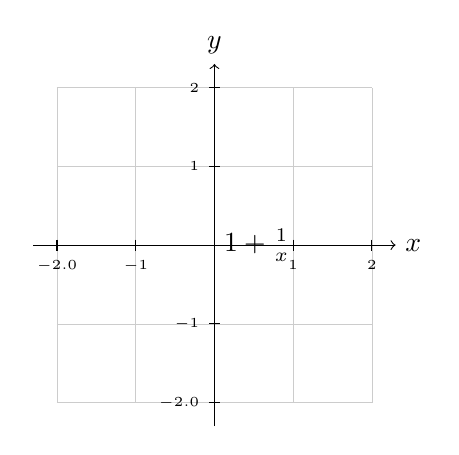
\begin{tikzpicture}
		[smooth]
		\pgfmathsetmacro\minx{-2}
		\pgfmathsetmacro\maxx{2}
		\pgfmathsetmacro\miny{-2}
		\pgfmathsetmacro\maxy{2}
		\draw[very thin,color=gray!40] (\minx,\miny) grid (\maxx,\maxy);
		\draw[->] (\minx-0.3,0) -- (\maxx+0.3,0) node[right] {$x$};
		\foreach \x in {\minx,...,-1}{\draw (\x cm,2pt) -- (\x cm,-2pt) node[below] {\tiny $\x$};}
		\foreach \x in {1,...,\maxx}{\draw (\x cm,2pt) -- (\x cm,-2pt) node[below] {\tiny $\x$};}
		\draw[->] (0,\miny-0.3) -- (0,\maxy+0.3) node[above] {$y$};
		\foreach \y in {\miny,...,-1}{\draw (2pt,\y cm) -- (-2pt,\y cm) node[left] {\tiny $\y$};}
		\foreach \y in {1,...,\maxy}{\draw (2pt,\y cm) -- (-2pt,\y cm) node[left] {\tiny $\y$};}
		\clip (\minx,\miny) rectangle (\maxx,\maxy);
		\draw[domain=-2:2,color=black] plot function{1+1/x} node[right] {$1+\frac{1}{x}$};
\end{tikzpicture}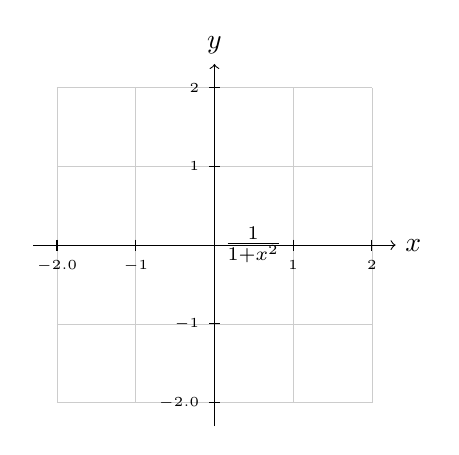
\begin{tikzpicture}
		[smooth]
		\pgfmathsetmacro\minx{-2}
		\pgfmathsetmacro\maxx{2}
		\pgfmathsetmacro\miny{-2}
		\pgfmathsetmacro\maxy{2}
		\draw[very thin,color=gray!40] (\minx,\miny) grid (\maxx,\maxy);
		\draw[->] (\minx-0.3,0) -- (\maxx+0.3,0) node[right] {$x$};
		\foreach \x in {\minx,...,-1}{\draw (\x cm,2pt) -- (\x cm,-2pt) node[below] {\tiny $\x$};}
		\foreach \x in {1,...,\maxx}{\draw (\x cm,2pt) -- (\x cm,-2pt) node[below] {\tiny $\x$};}
		\draw[->] (0,\miny-0.3) -- (0,\maxy+0.3) node[above] {$y$};
		\foreach \y in {\miny,...,-1}{\draw (2pt,\y cm) -- (-2pt,\y cm) node[left] {\tiny $\y$};}
		\foreach \y in {1,...,\maxy}{\draw (2pt,\y cm) -- (-2pt,\y cm) node[left] {\tiny $\y$};}
		\clip (\minx,\miny) rectangle (\maxx,\maxy);
		\draw[domain=-2:2,color=black] plot function{1/(x**2+1)} node[right] {$\frac{1}{1+x^2}$};
\end{tikzpicture}
\ul{Satz} Wenn $P(z) = \sum_{k \geq 0} a_k z^k$ ist eine Potenzreihe mit Konvergenzradius $R > 0$ ist, dann ist
\enum{
\item $P:(-R,R)→\R$ ∞ oft differenzierbar
\item $P=$Tailorreihe von $P$
}
\ul{Grund} Darf $P(z) = \sum_{k \geq 0} a_k z^k$ gliedweise ableiten:\\*
$P(z) = \sum_{k=1}^{\infty} k\cdot a_k z^{k-1}$ hat auch Konvergenzradius $R$\\*
$\frac{1}{1+x^2} = \frac{1}{1 - (-x^2)} = 1 + (-x^2) + (-x^2)^2 + (-x^2)^3 + ... $(geom. Reihe)\\
wenn $|x| < 1$ d.h. $|x| < 1 \Rarr \frac{1}{1+x^2} = 1 - x^2 + x^4 - x^6 ... = P(x)$\\
Konvergenzradius von $P$
\begin{tabular}{c|cccccc|c}
n&0&1&2&3&4&&\hline
\\$a_n$&1&0&-1&0&1&…&=1
\\$\sqrt[n]{|a_n|}$
&1&0&-1&0&1&…&\end{tabular}
Satz \Rarr{} Taylorreihe von $f(x) = \frac{1}{1 + x^2}$ ist $P(z)$ und hat den Konvergenzradius 1.\\*
\ul{Frage:} Wann konvergiert die Taylorreihe nicht weiter?
\ul{Antwort:} $z \mapsto \frac{1}{1 + x^2}$ ist eine Funktion $\C \setminus \{\pminus i\}$\\*
$1+z^z = 0 \equ z^z = -1 \equ z = \pminus i$\\*
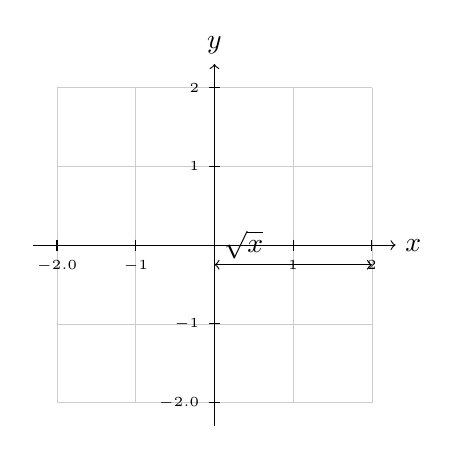
\begin{tikzpicture}
		[smooth]
		\pgfmathsetmacro\minx{-2}
		\pgfmathsetmacro\maxx{2}
		\pgfmathsetmacro\miny{-2}
		\pgfmathsetmacro\maxy{2}
		\draw[very thin,color=gray!40] (\minx,\miny) grid (\maxx,\maxy);
		\draw[->] (\minx-0.3,0) -- (\maxx+0.3,0) node[right] {$x$};
		\foreach \x in {\minx,...,-1}{\draw (\x cm,2pt) -- (\x cm,-2pt) node[below] {\tiny $\x$};}
		\foreach \x in {1,...,\maxx}{\draw (\x cm,2pt) -- (\x cm,-2pt) node[below] {\tiny $\x$};}
		\draw[->] (0,\miny-0.3) -- (0,\maxy+0.3) node[above] {$y$};
		\draw[<-] (0,-.25) -- (1,-.25);
		\draw[->] (1,-0.25) -- (2,-0.25);
		\foreach \y in {\miny,...,-1}{\draw (2pt,\y cm) -- (-2pt,\y cm) node[left] {\tiny $\y$};}
		\foreach \y in {1,...,\maxy}{\draw (2pt,\y cm) -- (-2pt,\y cm) node[left] {\tiny $\y$};}
		\clip (\minx,\miny) rectangle (\maxx,\maxy);
		\draw[domain=0.01:2,color=black] plot function{sqrt(x)} node[right] {$\sqrt{x}$};
\end{tikzpicture}
$R_{\geq 0} \R$ Taylorreihe von $a=1$ hat Konvergenzradius 1
1 = Konvergenzradius \Rarr{} $P$ definiert $\{|z| < 1\} \to \C$

\chapter{Newton Verfahren}
Gegeben $f:I→\R$, differnenzierbar\\*
suche Nullstellen\\*
Startwert $x_0$, Tangente an $x_0:\ T_1(x)=f(x_0)+(x-x_0)f'(x_0)$\\*
$x_1:=$Nullstelle von $T_1(x)$
\descr{Berechnung}{$T_1(x_1)=0$\\$f(x_0)+(x_1-x_0)f'(x_0)=0$
$$x_1-x_0=-\frac{f(x_0)}{f'(x_0)}$$
$$x_1:=x_0-\frac{f(x_0)}{f'(x_0)}$$
(geht nur wenn $f'(x)≠0$)\\*
Iterationen: $x_1:=x_n-\frac{f(x_0)}{f'(x_0)}$\\*
\sss{Frage}Konvergiert das gegen eine Nullstelle von $f$, wenn ja: wie schnell\\*
Annahme $f'(x)≠0\quad ∀x$
\bem
$f(x)=0\ \equ\ x=x-\frac{f(x_0)}{f'(x_0)}$, dass heißt (Nullstelle von $f$)=(Fixpunkte der Iteration $x\mapsto x-\frac{f(x_0)}{f'(x_0)}$)
\enum{
\item $f(x) = x + x^2$\\*
$f(0) = 0$\\*
$f'(x) = 1 + 2x\qquad x\mapsto x-\frac{f(x)}{f'(x)} = x - \frac{x+x^2}{1+2x} = \frac{x + 2x^2 - x - x^2}{1 + 2x} = \frac{x^2}{1 + 2x}$
\enum{
\item $x>0,\ x$ klein, dann $\frac{x^2}{1+2x}\approx x^2,\ \Rarr$ Folge $(x_n)$ mit $x_{n+1}=x_n-\frac{f(x_n)}{f'(x_n)}$ konvergiert schnell (quadratisch) gegen 0 (= Nullstelle)
\item $x>0,\ x$ groß dann $\frac{x^2}{1+2x}\approx \frac{x^2}{2x}=\frac{x}{2}$ 
}
\item $f(x) = x^2$\\
$x \mapsto x - \frac{f(x)}{f'(x)}$\\*
$= x - \frac{x^2}{2x} = x - \frac{x}{2} = \frac{x}{2} \Rarr (x_n) \to 0$\\
aber nicht quadratisch
\ul{Problem } $f'(0) = 0$ 
\item $f(x) = e^x - 1$\\*
$f(0) = 0$\\*
$f'(x) = e^x$\\*
$x \mapsto x - \frac{e^x - 1}{e^x} = x - 1 + \frac{1}{e^x}$\\*
Für $x > 0$ groß ist $x - 1 + \frac{1}{e^x} \approx x - 1$\\*
$x = 100$\\
$x_1 = 99$\\
$x_2 = 98$\\
$x_n = 0$ (NST)
aber langsam, solange $x_n$ nicht nahe an 0.
}